\section{Methodology}
\label{sec:method}

\subsection{Dataset}

The experiments use Mini-ImageNet, a 100-class image benchmark derived from ImageNet, composed of 50000 training images, 10000 validation images, and 5000 test images.

\paragraph{Preprocessing.}
Images are converted to RGB, resized to $392\times392$ using bicubic interpolation, and stored as unsigned 8-bit tensors while preserving splits and class labels; no cropping or data augmentation is performed.
These images are supplied to the native Qwen2.5-VL processor for teacher and probe extraction, while the ViT-B/16 evaluation transform independently produces the $224\times224$ student input.


\subsection{Teacher Probes}

We evaluate three probe heads: mean pooling with a linear classifier, learned attention pooling, and cross-attention pooling. Their role is to provide meaningful class-discriminative gradients from which token saliency can be computed.

\paragraph{Probe details.}
The probe backbone is the frozen visual module of Qwen2.5-VL-3B-Instruct.
Only the probe heads are trained, while the backbone is frozen.
For an image, let $T=[t_1,\ldots,t_N]^\top \in \mathbb{R}^{N\times d}$ denote the sequence of frozen visual tokens.
Each probe first produces an image representation $h\in\mathbb{R}^{d}$ and then applies the same form of linear classification, $y=Wh+b$, where $y\in\mathbb{R}^{100}$ contains the Mini-ImageNet logits.
Here, $W$ and $b$ are the trainable classifier parameters.
The mean probe has no learnable pooling parameters and computes
\begin{equation}
  h_{\mathrm{mean}}=\frac{1}{N}\sum_{i=1}^{N}t_i.
\end{equation}
For additive-attention pooling, normalized tokens $\bar{t}_i=\operatorname{LN}(t_i)$ are scored by a two-layer network,
\begin{equation}
  \begin{aligned}
    e_i &= w_2^\top\operatorname{GELU}(W_1\bar{t}_i+b_1)+b_2, \\
    \alpha_i &= \operatorname{softmax}(e)_i, &
    h_{\mathrm{attn}} &= \sum_{i=1}^{N}\alpha_i\bar{t}_i ,
  \end{aligned}
\end{equation}
Here, $W_1,b_1,w_2,b_2$ are trainable scorer parameters, $e_i$ is the scalar score assigned to token $i$, and $\alpha_i$ is its normalized pooling weight.
The scorer hidden dimension is $\max(64,\lfloor d/4\rfloor)$.
The cross-attention probe instead introduces a single learned query $q\in\mathbb{R}^{d}$ and pools the normalized token sequence through multi-head attention:
\begin{equation}
  h_{\mathrm{cross}}=
  \operatorname{MHA}\!\left(q,\operatorname{LN}(T),\operatorname{LN}(T)\right).
\end{equation}
where $\operatorname{MHA}$ denotes standard multi-head attention and $q$ is its trainable pooling query.

\begin{figure*}[t]
  \centering
  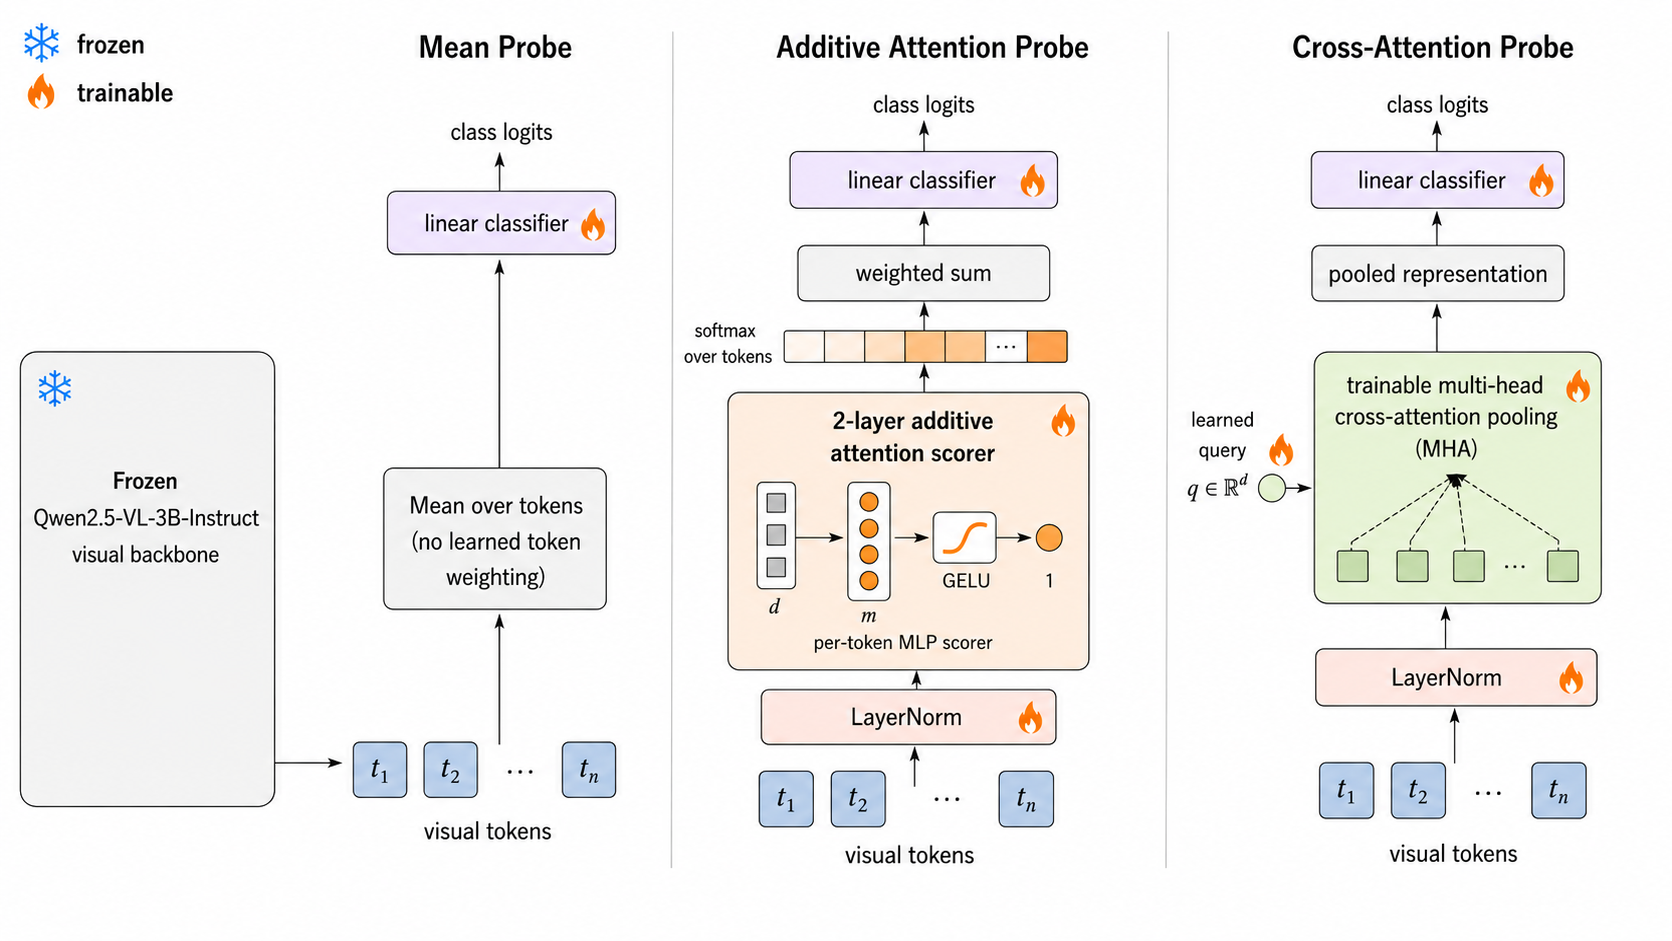
\includegraphics[width=0.96\textwidth]{figures/probes.png}
  \caption{Probe-head architectures tested.}
  \label{fig:probe-heads}
\end{figure*}

All probe classifiers use zero dropout at the classification head.
Probe training uses AdamW for 10 epochs with batch size 16, learning rate $3\times10^{-4}$, weight decay 0.01, warmup ratio 0.1, cosine learning-rate decay, gradient clipping at norm 1.0 and seed 42 for reproducibility.
The checkpoint used for saliency computation is the best one on the validation set.

\paragraph{Grad-CAM token weights.}
For each image, the frozen Qwen visual backbone produces a token sequence $\{t_i\}_{i=1}^N$.
A trained probe reads these tokens and predicts logits.
We take the class predicted by the probe and ask which visual tokens most supported that logit.
To answer this, Grad-CAM backpropagates the selected logit through the probe head and classifier to the visual tokens.

Because the visual backbone is fixed, differences among the resulting Grad-CAM maps arise from the trained pooling and classification paths from $T$ to the selected logit.

For each probe we backpropagate the target logit through the probe and compute a token-level Grad-CAM score
\begin{equation}
  c_i = \operatorname{ReLU}\left(\sum_d
  \frac{\partial y_k}{\partial t_{i,d}}\,t_{i,d}\right),
\end{equation}
where $y_k$ is the logit of the probe-predicted class and $d$ indexes the feature dimensions of token $t_i$.
The raw scores are normalized per image and sharpened with a softmax temperature $\tau=0.05$ to obtain the final token weights $A_i$.
If the scores are degenerate or non-finite, the example falls back to uniform token weights.
% The probe returns one relevance weight for each location in its Qwen token map.
% Because this map is denser than the student token map, the weights are resized before they are used in distillation.

\subsection{Distillation}

\paragraph{Matching teacher and student tokens.}
The probe and the student initially describe the image at different spatial granularities.
At the resolution used in the experiments, the probe assigns relevance weights on a $28\times28$ Qwen token map, while the ViT-B/16 student produces $14\times14=196$ patch tokens from its $224\times224$ input.
We resize the probe relevance map to $14\times14$ and normalize the resulting 196 weights to sum to one.

The teacher target is Qwen's sequence of 196 image embeddings: these are the visual representations normally provided to the language model when it generates an answer.
The student also produces 196 token embeddings, and a learned linear projection maps each student token to the dimension of the teacher.

We compare three distillation objectives.
The baseline aligns the mean visual embedding of the student and teacher using a mean-squared error loss:
\begin{equation}
  \mathcal{L}_{global} = \left\lVert \frac{1}{N}\sum_{i=1}^{N} s_i - \frac{1}{N}\sum_{i=1}^{N} t_i \right\rVert_2^2.
\end{equation}
where $N$ is the number of aligned visual token locations, $t_i$ is the Qwen teacher embedding at location $i$, $s_i$ is the projected student embedding at the same location, and $A_i$ is the resized and normalized relevance weight assigned to location $i$.
The explanation-guided objective uses the aligned token-level weights $A_i$ to concentrate supervision on salient teacher regions:
\begin{equation}
  \mathcal{L}_{expl} = \sum_{i=1}^{N} A_i \left\lVert s_i - t_i \right\rVert_2^2.
\end{equation}
The combined loss is a weighted sum,
\begin{equation}
  \mathcal{L} = \lambda_g\,\mathcal{L}_{global} + \lambda_e\,\mathcal{L}_{expl},
\end{equation}
where $\lambda_g, \lambda_e \ge 0$ control the balance between global reconstruction and explanation-weighted local matching. 

We evaluate three settings: (1) $\lambda_g=1, \lambda_e=0$ (global MSE baseline); (2) $\lambda_g=0, \lambda_e=1$ (explanation-only local matching); and (3) $\lambda_g=1, \lambda_e=1$ (combined objective).

% \begin{table}[t]
%   \centering
%   \caption{Distillation variants. The main ablation is whether the student uses only global reconstruction, only explanation-guided token matching, or both.}
%   \label{tab:variants}
%   \small
%   \begin{tabular}{@{}lll@{}}
%     \toprule
%     Variant & Saliency source & Objective \\
%     \midrule
%     Base MSE & none & global MSE \\
%     Mean expl. & mean probe & explanation only \\
%     Attn expl. & attention probe & explanation only \\
%     Cross expl. & cross-attn probe & explanation only \\
%     Mean MSE+expl. & mean probe & global + explanation \\
%     Attn MSE+expl. & attention probe & global + explanation \\
%     Cross MSE+expl. & cross-attn probe & global + explanation \\
%     \bottomrule
%   \end{tabular}
% \end{table}

Teacher features and token weights are precomputed before student training.
For the global MSE baseline, the teacher is the vision part of Qwen2.5-VL-3B.
For explanation-guided variants, the teacher is the validation-best probe checkpoint and token weights are Grad-CAM saliency weights derived from the probe logits.
The student is a ViT-B/16 at 224-pixel resolution, followed by a projection into the teacher feature dimension.

\paragraph{Distillation training details.}
Student training uses AdamW for at most 20 epochs with train batch size 16, precompute batch size 4, learning rate $3\times10^{-4}$, weight decay 0.05, warmup ratio 0.1, cosine learning-rate decay, gradient clipping at norm 1.0 and seed 42 for reproducibility.
% Validation and test distillation losses are evaluated every epoch.
Early stopping monitors validation distillation loss with patience 5; reported results use the validation-best student checkpoint.
% The explicit coefficient settings are the three rows in Table~\ref{tab:variants}: $(\lambda_g,\lambda_e)=(1,0)$ for the baseline, $(0,1)$ for explanation-only distillation, and $(1,1)$ for the combined objective.

\subsection{Evaluation Metrics}
\label{sec:metrics}


We report three families of metrics. First, teacher probes are measured by validation accuracy and test accuracy. Second, student distillation is measured on validation and test sets using the loss objectives defined above: global MSE, explanation-weighted MSE, and the combined loss. Third, downstream VLM behavior is measured through generated-answer comparison, using an LLM jury: independent VLM judges see the original image and two anonymized answers (that are, the student and teacher answers), then select the better answer or a tie, without any information about which answer is from the teacher or the student. We report majority preference over the three judges on examples where all judges return valid structured outputs. For the judge panel, we employ the \emph{all-judge agreement} as the fraction of examples where all three judges select the same class, and Fleiss' $\kappa$ estimates agreement to measure inter-judge reliability beyond chance. The judge panel is made up of three local VLMs: Qwen3.5-9B~\citep{qwen2026qwen35}, GLM-4.6V-Flash~\citep{vteam2025glm45v}, and MiniCPM-V-4.5~\citep{yu2025minicpmv45}.
Each LLM is loaded with a context length of 32,768 and temperature 0.0.
The generated teacher and student answers are capped at 128 new tokens before judging.
Both text-only and image-grounded judges are constrained to return a structured JSON.
We report the results considering only the subset of examples where all three judges return a valid structured preference.
